% Build with XeLaTeX (Tectonic: `tectonic -X compile report.tex`; Overleaf: set
% the compiler to XeLaTeX). The Japanese example needs a CJK font.
\documentclass[11pt]{article}
\usepackage[margin=2.0cm]{geometry}
\usepackage{fontspec}
% Atkinson Hyperlegible was designed by the Braille Institute for legibility:
% open letter shapes, a large x-height, and distinct I/l/1 and O/0.
\setmainfont{Atkinson-Hyperlegible}[Extension=.otf, UprightFont=*-Regular-102,
  BoldFont=*-Bold-102, ItalicFont=*-Italic-102, BoldItalicFont=*-BoldItalic-102]
\usepackage{xeCJK}
\IfFontExistsTF{Hiragino Sans W4}{\setCJKmainfont{Hiragino Sans W4}}{\setCJKmainfont{Noto Sans CJK JP}}
\usepackage{graphicx,booktabs,amsmath,xcolor,caption,float,enumitem,makecell,wrapfig}
\renewcommand{\theadfont}{\small\bfseries}
\usepackage[numbers]{natbib}
\usepackage{hyperref}
\captionsetup{font=small,labelfont=bf}
\setlength{\parskip}{0.3em}
\setlength{\parindent}{0pt}
\raggedbottom
\linespread{1.04}
\setlist{itemsep=1pt,topsep=2pt}
\hypersetup{colorlinks=true,linkcolor=black,citecolor=blue!50!black,urlcolor=blue!50!black}
\newcommand{\finding}[1]{\par\noindent\textbf{Finding: #1}\par}


\begin{document}
\begin{center}
{\LARGE\bfseries How Good Can a Japanese Language Model\\[3pt]
Get in 30 GPU-Minutes?\par}
\vspace{8pt}
{\large Tokenization, model size and repeated data under a fixed budget\par}
\vspace{14pt}
{\large Madrid Lim\par}
\vspace{3pt}
Student ID A0307648W \quad$\cdot$\quad
\href{mailto:e1398088@u.nus.edu}{e1398088@u.nus.edu}
\end{center}
\vspace{4pt}

\begin{abstract}
\noindent I train small Japanese language models from random weights, giving
each model exactly 30 minutes of training on one GPU, and ask how to spend that
budget. Across 12 such runs I find that: (1) splitting text into learned word
pieces (BPE) beats splitting it into characters or raw bytes; (2) the best model size is 10--25 million parameters, and the best single model
read 15--24 tokens of text per parameter, consistent with the rule of thumb of
\citet{hoffmann2022chinchilla};
and (3) for film-subtitle text, adding subtitles to the training mix helps
far more than adding Wikipedia, and repeating the same 24 million subtitle
tokens 11 times still helped slightly. I also test whether a model's surprise
at a sentence can rate its difficulty for learners of Japanese. It does not help: adding the model's surprise to sentence length does not
measurably improve predictions of a sentence's JLPT level, while adding the
share of kanji does. All code, configurations and results are at
\url{https://github.com/StarlightsJourney/tiny-japanese-lm}.
\end{abstract}

\section{Declared setup}

The project brief asks for three things to be fixed before any experiment.
Table~\ref{tab:setup} states them.

\begin{table}[H]
\centering\small
\begin{tabular}{p{0.2\linewidth}p{0.74\linewidth}}
\toprule
\textbf{Compute budget} & 30 minutes (1{,}800\,s) of training per run on one NVIDIA
L4 GPU (24\,GB), rented from Modal. The clock runs only while the model is
learning: reading a batch of text, measuring its errors and updating its
weights. One such update is a \emph{training step}. Pausing to score held-out
text is not counted, so measuring progress never costs training time. Not
counted either, as the brief allows: data preparation, tokenizer training and a
preliminary learning-rate search (Section~\ref{sec:lr}). \\
\addlinespace
\textbf{Initialisation} & Every model starts from random weights. No pretrained
weights, embeddings or other pretrained components are used. The tokenizers are
trained on my own training data. \\
\addlinespace
\textbf{Evaluation objective} & \emph{Data:} held-out Japanese film and TV
subtitles (primary) and held-out Japanese Wikipedia (secondary), never seen in
training. \emph{Metric:} bits per byte (BPB), defined in
Section~\ref{sec:bpb}; lower is better. \emph{Why:} BPB measures how well the
model predicts real text it has not seen, which is what a language model is
for. It is measured per byte of text rather than per token, so models that cut
text into different pieces are compared on equal terms. Subtitles are primary
because the model is meant for an app whose users learn from films and TV.
\emph{Protocol:} choices are made on a validation set; final numbers come from
a separate test set. Every model is scored on the same subtitle test text. \\
\bottomrule
\end{tabular}
\caption{The declared budget, initialisation and evaluation objective.}
\label{tab:setup}
\end{table}

\section{Motivation}

I am building Sheng, an offline desktop app for learning Japanese from films
and TV. It shows live subtitles and lets the user save sentences as flashcards.
It would help to know how hard each sentence is, so the app can point out lines
just above the learner's level. This must run offline on a laptop, so any model
has to be small. A language model is a natural candidate: if a sentence
surprises the model, it might surprise a learner too. That raises two
questions. How good a Japanese model can be trained cheaply, and how should the
budget be spent? And is the model's surprise useful as a difficulty score?

\section{Background and terms}

\textbf{Language model and loss.} A language model reads text as a sequence of
\emph{tokens} and, at each position, assigns a probability to every possible
next token. Training adjusts the model's \emph{parameters} (its weights) to make
the true next token more probable. The quantity minimised is the \emph{cross-entropy loss}: the average of
$-\ln p(\text{true next token})$. It is measured in nats per token (a nat is the
natural-log unit of information; 1 nat $\approx$ 1.44 bits). It measures
surprise: a model that always gives the true token probability 1 has loss 0.

\textbf{Bits per byte.}\label{sec:bpb} Loss per token cannot compare tokenizers:
a tokenizer with longer tokens makes fewer, harder predictions over the same
text. So I convert the total loss on a text into bits and divide by the text's
length in UTF-8 bytes:
\[
\text{BPB} = \frac{\sum_{\text{tokens}} -\log_2 p(\text{true next token})}{\text{number of UTF-8 bytes in the text}} .
\]
This is the measure used for The Pile \citep{gao2020pile}. It is roughly the size, per byte, that the text would compress to using the
model's predictions. Most Japanese characters take 3 bytes in UTF-8, and the
subtitles average 2.8 bytes per character, so 1.33 BPB is about 3.7 bits per
character.

\textbf{What BPB leaves out.} It measures prediction only. It says nothing about
whether text the model generates is fluent or correct, or whether the model is
useful for a downstream task (Section~\ref{sec:diff} tests one such task
separately). It averages over all bytes, so common patterns dominate the score.
And its absolute differences look small: a gain of 0.01 BPB is under 1\% of the
total.

\textbf{Tokenizers.} A tokenizer decides what the units of text are. I compare
four (Table~\ref{tab:tokex}). \emph{Byte}: every UTF-8 byte is a token, so one
Japanese character becomes three tokens. \emph{Char}: every character is a
token. \emph{BPE} (byte-pair encoding, \citealp{sennrich2016bpe}): start from
bytes and repeatedly merge the most frequent adjacent pair into a new token,
until the vocabulary reaches a set size. The result is a vocabulary of common
word pieces; I use the byte-level version of \citet{radford2019gpt2} with 4{,}096
or 16{,}384 tokens. Longer tokens mean each prediction covers more text. The cost is a larger
vocabulary: the model learns one vector (an \emph{embedding}) per token, so a
larger vocabulary means more parameters and a larger final layer.

\begin{table}[H]
\centering\small
\begin{tabular}{lrl}
\toprule
Tokenizer & Tokens & How 心配しないで、俺がやるから。 (``Don't worry, I'll do it.'') is split \\
\midrule
byte   & 42 & \texttt{e5|bf|83|e9|85|8d|e3|81|97|}\ldots{} (one token per byte) \\
char   & 14 & 心|配|し|な|い|で|、|俺|が|や|る|か|ら|。 \\
bpe4k  & 8  & 心配|しない|で|、|俺が|やる|から|。 \\
bpe16k & 7  & 心配|しないで|、|俺が|やる|から|。 \\
\bottomrule
\end{tabular}
\caption{One subtitle-style sentence (42 bytes) cut by each tokenizer, using
the tokenizers trained in this project. With 16k tokens, しないで (``don't'')
becomes a single token.}
\label{tab:tokex}
\end{table}

\textbf{Budgets.} \citet{kaplan2020scaling} found that loss falls smoothly as
parameters, data and compute grow. \citet{hoffmann2022chinchilla} found that
for a fixed amount of compute, parameters and training tokens should grow
together, at about 20 tokens per parameter. Training compute is roughly
$C \approx 6ND$ floating-point operations (FLOPs) for $N$ parameters and $D$
tokens. Their models had 70M to 16B parameters; whether the ratio holds for a few
million is untested. \citet{muennighoff2023scaling} studied the case where unique
text runs out. They found that up to about four \emph{epochs} (passes over the
same data) is almost as good as fresh data, with value decaying after that.
Japanese subtitles are such a scarce source.

\textbf{Surprise and difficulty.} Surprisal theory holds that the surprise of a
word under a probabilistic language model predicts how hard it is for people to
read \citep{hale2001probabilistic,levy2008expectation}. Language-model scores
have also been used to rate text readability without labelled data
\citep{martinc2021readability}. For learners of Japanese,
\citet{benedetti2025examples} use pretrained language models to suggest example
sentences. My question is
whether a tiny model trained from scratch carries any of this signal.

\section{Method}

\subsection{Data}

\textbf{Subtitles} are the Japanese side of JESC \citep{pryzant2018jesc}, 2.8M
lines. I normalise each line, drop lines with no Japanese characters, and
remove exact duplicates, because subtitles repeat short lines such as ``hai''
(``yes'') constantly and a line in both training and test data would inflate
test scores. A hash of each line sends it to training, validation or test
(99/0.5/0.5), so the split never changes. \textbf{Wikipedia} is the first
$\sim$600\,MB of the November 2023 Japanese dump; each article goes wholly to
one split. Table~\ref{tab:data} gives the sizes.

\begin{table}[H]
\centering\small
\begin{tabular}{lrrrr}
\toprule
\thead{Source} & \thead{Train\\lines} & \thead{Train\\text} & \thead{Validation / test\\lines} & \thead{Validation / test\\text} \\
\midrule
Subtitles (JESC) & 2{,}476{,}413 & 118.5\,MB & 12{,}564 / 12{,}683 & 0.61 / 0.61\,MB \\
Wikipedia (Japanese) & 3{,}097{,}333 & 561.8\,MB & 14{,}707 / 20{,}765 & 2.96 / 3.82\,MB \\
\bottomrule
\end{tabular}
\caption{Data after cleaning and splitting.}
\label{tab:data}
\end{table}


\subsection{Model and training}

The model is a decoder-only transformer \citep{vaswani2017attention}, the
architecture of GPT-style models, adapted from nanoGPT
\citep{karpathy2022nanogpt}. It reads 512 tokens at a time
(its \emph{context}) and is trained on batches of 64 such sequences. Weights are updated with AdamW \citep{loshchilov2019adamw}, a standard
optimiser. Each sequence is drawn from
subtitles with a fixed probability, the \emph{subtitle share}. By default this
is the natural share: the fraction of all training tokens that are subtitles,
16\% for BPE-16k. The \emph{learning rate} sets how large each update is. It
rises over the first 2\% of the budget, then falls smoothly to 10\% of its peak
by the end. The schedule follows elapsed time rather than step count, because
under a time budget the number of steps is not known in advance.

I compare four model sizes: \textbf{xs}, \textbf{s}, \textbf{m} and \textbf{l},
with 4, 6, 8 and 12 layers and 3.2M, 10.6M, 25.2M and 59.0M parameters, not
counting the token embeddings. The \emph{baseline} is size s with BPE-16k and
the natural subtitle share. Each experiment changes one thing from the baseline.

\subsection{Learning-rate search}\label{sec:lr}

A learning rate that suits one model size can be too high for another, so a
single rate would have handicapped some sizes. I chose each size's peak rate
with 6-minute runs, picking the best validation BPB. My first guesses were too
high for s, m and l: each preferred the lowest rate tried. I extended the search
downwards until every chosen rate had a worse rate on both sides
(Appendix~\ref{app:lr}). The search mattered. The baseline's tuned rate scored
0.028 BPB better than my first guess, more than several effects reported below.

\subsection{Evaluation details}

Validation BPB is measured every 2 minutes on up to 200k tokens per source.
Test BPB is measured once, at the end, on up to 2M tokens per source. Every
model scores the whole subtitle test set. Two caps affect what text is scored.
Validation uses the first 200k tokens, which is less text for tokenizers with
short tokens. And the byte model's Wikipedia test score covers only the first
2.0\,MB of 3.8\,MB. Comparisons between tokenizers therefore rest on the
subtitle test set.

\section{Results}

Figure~\ref{fig:curves} shows how every model improved during training. All
results are single runs except the baseline, which was run with three random
seeds to measure noise.

\begin{figure}[H]
\centering
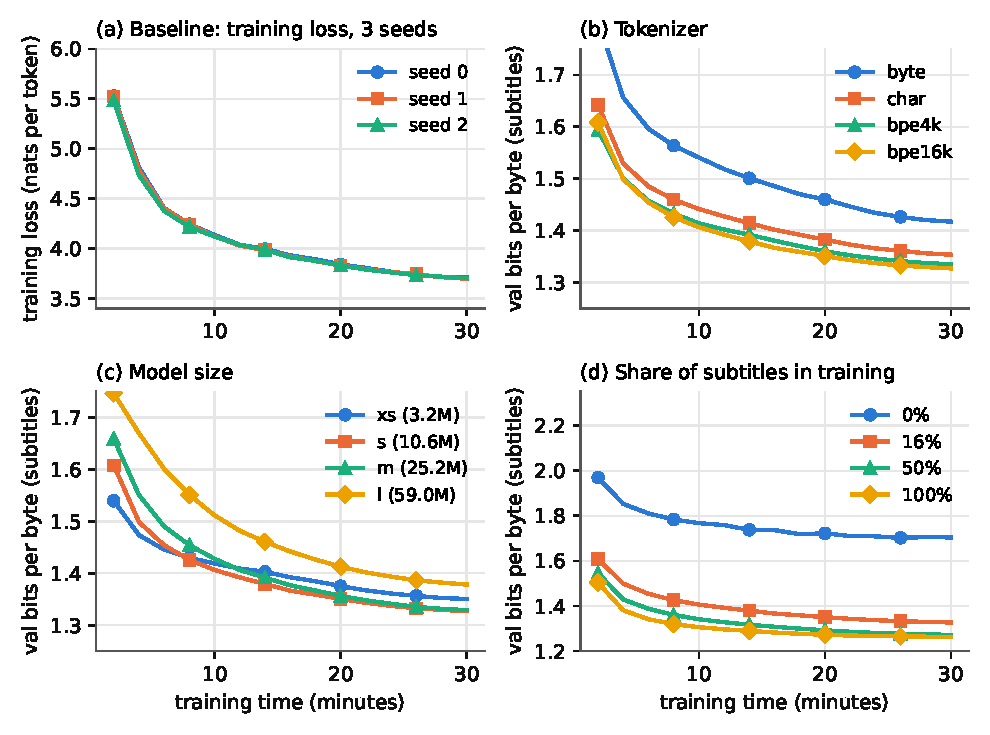
\includegraphics[width=0.8\linewidth]{figures/curves.pdf}
\caption{Learning curves. (a) The training loss of the baseline, for three
random seeds. (b)--(d) Validation BPB on subtitles during training, for each
experiment. Every model was still improving when its 30 minutes ran out.}
\label{fig:curves}
\end{figure}


\subsection{How much do results vary between runs?}

\finding{the noise between runs is about 0.0015 BPB, much smaller than most
effects studied here.}

The three baseline seeds gave test BPB of 1.3343, 1.3326 and 1.3313 on
subtitles (standard deviation 0.0015) and validation BPB of 1.3270, 1.3251 and
1.3251 (standard deviation 0.0011). The seed changes the random starting weights
and the order of training batches. Under a time budget, the GPU's speed also
matters: these runs processed between 141k and 145k tokens per second. Their
training losses are almost indistinguishable (Figure~\ref{fig:curves}a). When
two single runs differ by less than about three standard deviations of their
difference ($3\times\sqrt{2}\times0.0011 \approx 0.005$ BPB on validation), I
treat them as tied. Three seeds give only a rough estimate of the noise, so I
rely on gaps near this threshold only when other evidence agrees.

\subsection{Tokenizer}

\finding{learned word pieces beat characters, and characters beat bytes. BPE-16k
is best.}

The byte model processes the most tokens per second, but each token is one byte,
so in 30 minutes it reads the least text, and its 512-token context holds only
about 170 Japanese characters (Table~\ref{tab:tok}). Characters and BPE tokens
each cover more text, so those models read more and see more context at once.

\begin{table}[H]
\centering\small
\begin{tabular}{lrrrrrr}
\toprule
\thead{Tokenizer} & \thead{Total\\params} & \thead{Tokens\\per second} & \thead{Text read\\in 30 min} & \thead{Text in one\\context} & \thead{Test BPB,\\subtitles} & \thead{Test BPB,\\Wikipedia} \\
\midrule
byte   & 10.9M & 264k & 0.48\,GB & 512\,B   & 1.430 & 1.327 \\
char   & 12.9M & 206k & 1.00\,GB & 1.4\,KB & 1.362 & 1.205 \\
bpe4k  & 12.4M & 217k & 1.41\,GB & 2.1\,KB & 1.344 & 1.173 \\
bpe16k & 17.1M & 141k & 1.17\,GB & 2.6\,KB & \textbf{1.334} & \textbf{1.156} \\
\bottomrule
\end{tabular}
\caption{Tokenizer comparison (size s, 30 minutes each). ``Total params''
includes the token embeddings, which grow with the vocabulary.}
\label{tab:tok}
\end{table}


BPE-16k beats BPE-4k by 0.008 on validation, 0.010 on the subtitle test and
0.017 on the Wikipedia test. The validation gap is above the noise threshold,
and both test sets agree, so I take it as real. It is not because BPE-16k read
more: its larger output layer makes it the slowest model, and it read 1.17\,GB
of text against 1.41\,GB for BPE-4k. Two differences remain that could explain
it. Its context covers more text (2.6\,KB against 2.1\,KB), and its embedding
table adds 6.3M parameters, against 1.6M for BPE-4k. I held the non-embedding
size fixed, as is usual, but this means the larger vocabulary also had more
parameters in total. My experiments cannot separate these two causes.

\subsection{Model size}

\finding{the best size is a flat region between 10M and 25M parameters. The best
model read 15--24 tokens per parameter.}

The smallest model read the most text, 128 tokens per parameter, and still did
worse than s (Table~\ref{tab:size}): it lacks the capacity to use the data. The
largest model read only 1.5 tokens per parameter and did worst: it is far from
trained. Sizes s and m differ by 0.002 on validation, below the noise threshold,
so they tie.

\begin{table}[H]
\centering\small
\begin{tabular}{lrrrrrrr}
\toprule
\thead{Size} & \thead{Params\\(non-emb.)} & \thead{Params\\(total)} & \thead{Peak\\learning rate} & \thead{Tokens\\read} & \thead{Tokens per\\param} & \thead{Val BPB,\\subtitles} & \thead{Test BPB,\\subtitles} \\
\midrule
xs & 3.2M  & 7.5M  & $3\times10^{-3}$   & 404M & 128 & 1.351 & 1.358 \\
s  & 10.6M & 17.1M & $1\times10^{-3}$   & 254M & 24  & \textbf{1.327} & \textbf{1.334} \\
m  & 25.2M & 33.8M & $7.5\times10^{-4}$ & 161M & 6.4 & 1.329 & 1.336 \\
l  & 59.0M & 69.8M & $5\times10^{-4}$   & 89M  & 1.5 & 1.378 & 1.386 \\
\bottomrule
\end{tabular}
\caption{Model-size comparison (BPE-16k, natural subtitle share). Tokens per
parameter uses non-embedding parameters.}
\label{tab:size}
\end{table}


The winner, s, read 24 tokens per non-embedding parameter, or 15 per parameter
if the embedding table is counted. Both are close to the $\sim$20 of
\citet{hoffmann2022chinchilla}. Their rule, $N \approx \sqrt{C/120}$, predicts
an optimal size of about 15M parameters for this run's $2.6\times10^{16}$ FLOPs.
s has 17.1M in total. This is one budget and four sizes, so it is consistent
with their rule rather than a test of it.

\begin{wrapfigure}[13]{r}{0.46\linewidth}
\vspace{-12pt}
\centering
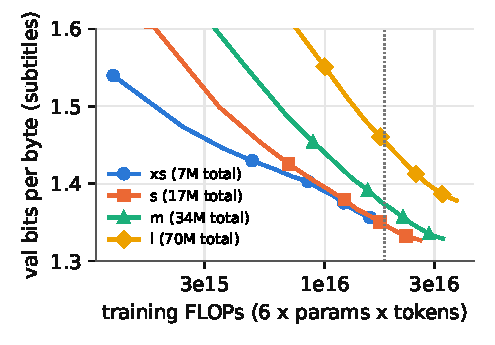
\includegraphics[width=\linewidth]{figures/compute.pdf}
\caption{Validation BPB against compute. Dotted line: all the compute xs used.}
\label{fig:compute}
\vspace{-10pt}
\end{wrapfigure}
\textbf{Equal time is not equal compute.} Larger models make better use of the
GPU, so in the same 30 minutes l performed about twice the computation of xs
($3.7$ against $1.8\times10^{16}$ FLOPs). Figure~\ref{fig:compute} plots the
same runs against compute instead of time. At $1.8\times10^{16}$ FLOPs, all xs
used, validation BPB is 1.351 (xs), 1.347 (s), 1.374 (m) and 1.455 (l). At equal
compute, s now clearly beats m. This suggests that a time budget favours larger
models somewhat. The comparison is not exact, though: m and l are read off
part-way through their runs, before their learning rates had finished
decreasing, which makes them look worse than a run planned for that compute
would.




\subsection{Data mix and repetition}

\finding{for subtitle text, subtitles in training matter far more than
Wikipedia, and repeating them 11 times still helped slightly.}

A model trained only on Wikipedia scores 1.718 on subtitles. Moving 16\% of
training to subtitles improves that by 0.38, the largest effect in this study
(Table~\ref{tab:data_mix}, Figure~\ref{fig:datamix}). Each further
increase helps less: 0.055 from 16\% to 50\%, and 0.008 from 50\% to 100\%. The
last gain is small but above the noise threshold. It comes from reading the
same 24M subtitle tokens 10.8 times, well beyond the four passes that
\citet{muennighoff2023scaling} found to be nearly as good as new data.

\begin{table}[H]
\centering\small
\begin{tabular}{lrrrr}
\toprule
\thead{Subtitle\\share} & \thead{Passes over\\subtitles} & \thead{Test BPB,\\subtitles} & \thead{Test BPB,\\Wikipedia} & \thead{Validation $-$\\training gap} \\
\midrule
0\%            & 0    & 1.718 & \textbf{1.144} & 0.040 \\
16\% (natural) & 1.7  & 1.334 & 1.156 & 0.035 \\
50\%           & 5.5  & 1.279 & 1.203 & 0.034 \\
100\%          & 10.8 & \textbf{1.270} & 2.447 & 0.100 \\
\bottomrule
\end{tabular}
\caption{Data-mix comparison (size s, BPE-16k). The last column is validation
BPB minus training BPB at the end of the run, over the run's own mix of sources;
the 16\% value is the mean of three seeds.}
\label{tab:data_mix}
\end{table}

\begin{wrapfigure}{r}{0.46\linewidth}
\vspace{-12pt}
\centering
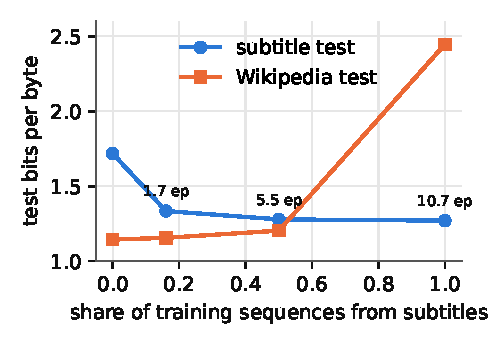
\includegraphics[width=\linewidth]{figures/data.pdf}
\caption{Test BPB as the subtitle share grows, labelled with passes (epochs)
over the subtitle data.}
\label{fig:datamix}
\vspace{-10pt}
\end{wrapfigure}
Repetition did leave a trace. The gap between validation and training BPB, a
sign of memorisation, stays at 0.034--0.040 up to 5.5 passes, including the run
with no subtitles at all. At 10.8 passes it rises to 0.100. This suggests the
model has begun to memorise repeated lines, though its validation score was
still improving when training ended (Figure~\ref{fig:curves}d). In the 50\% run
the gap is averaged over both sources, so memorisation of subtitles there could
be hidden by the Wikipedia half.

Specialising costs general ability. On Wikipedia, the 50\% model is 0.047
worse than the baseline, and the subtitles-only model's BPB more than doubles (2.447 against 1.156). For an
app that sees only subtitles, the 50\% mix keeps most of the subtitle gain
while staying usable on other Japanese text.

\subsection{Does surprise track difficulty?}\label{sec:diff}

\finding{model surprise adds nothing measurable to sentence length. Length plus
kanji share is the better difficulty score.}

\textbf{Test set.} I took Japanese sentences of 5--40 characters from Tatoeba
\citep{tatoeba}, split them into words with fugashi \citep{mccann2020fugashi},
and labelled each with the JLPT level of its hardest word, using open JLPT word
lists \citep{jlptdecks}. The JLPT is the standard Japanese proficiency test, with
levels from N5 (easiest) to N1 (hardest). I kept 400 sentences per level. Each
sentence is scored by its BPB under the model. I measure agreement with level by
Spearman's $\rho$, a correlation of rankings: $+1$ means harder sentences always
score higher, and 0 means no relation.

Model BPB barely tracks level ($\rho$ = 0.05--0.12, top row of Table~\ref{tab:diff}),
while sentence length alone reaches 0.27 and kanji share 0.21.
Figure~\ref{fig:diff} shows why. The easiest sentences have the highest BPB,
and the easiest sentences are also the shortest. Across all sentences, BPB
falls as length grows ($\rho = -0.27$ for the baseline). A likely reason is
that the start of any sentence is hard to predict, and in a short sentence the
start is a large share of the bytes. Two effects pull in opposite directions:
harder words raise BPB, and the greater length of hard sentences lowers it.

\begin{figure}[H]
\centering
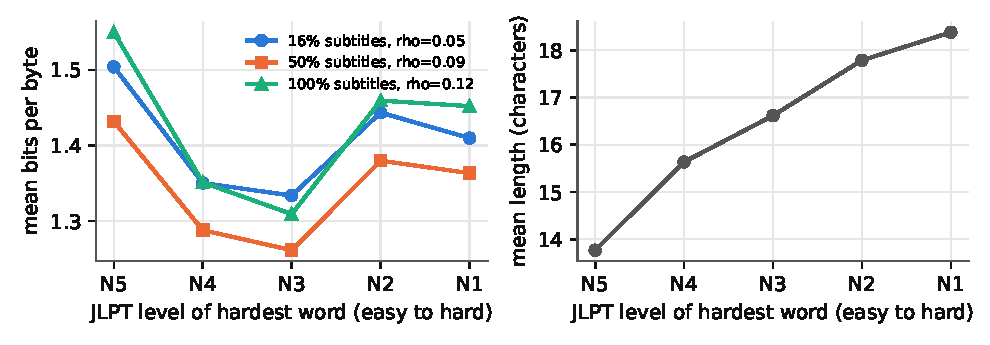
\includegraphics[width=0.96\linewidth]{figures/difficulty.pdf}
\caption{Left: mean BPB of the difficulty-set sentences at each JLPT level, for
models trained with 16\%, 50\% and 100\% subtitles. Right: mean sentence length
at each level.}
\label{fig:diff}
\end{figure}


Holding length fixed reveals a real but weak link between BPB and level,
$\rho \approx 0.13$--$0.17$, with intervals well above zero. The models trained
on more subtitles score slightly higher, but their intervals overlap, so I
cannot claim a trend.

\begin{table}[H]
\centering\small
\begin{tabular}{lrrr}
\toprule
Score (Spearman $\rho$ with JLPT level) & 16\% subtitles & 50\% subtitles & 100\% subtitles \\
\midrule
Model BPB & 0.05 & 0.09 & 0.12 \\
Model BPB, with length held fixed (95\% interval) & 0.13 (0.09--0.18) & 0.16 (0.11--0.20) & 0.17 (0.12--0.21) \\
\midrule
\multicolumn{4}{l}{\emph{Score fitted on 80\% of sentences, tested on the other 20\% (5-fold):}} \\
Length & 0.26 & 0.26 & 0.26 \\
Length + model BPB & 0.27 & 0.27 & 0.27 \\
Length + kanji share & \textbf{0.36} & \textbf{0.36} & \textbf{0.36} \\
Length + kanji share + model BPB & 0.36 & 0.36 & 0.36 \\
\bottomrule
\end{tabular}
\caption{Difficulty results on 2{,}000 Tatoeba sentences. Length and kanji
share do not depend on the model, so their rows repeat across columns.}
\label{tab:diff}
\end{table}


The practical test is whether the model improves a prediction that free
features already make. It does not. Fitted on part of the data and tested on
the rest, length alone gives $\rho = 0.26$, and adding model BPB raises it by
only 0.004--0.006 (for the baseline, 95\% interval $-0.003$ to $+0.016$). Adding
kanji share instead raises it to 0.36, and adding the model on top of that
changes nothing.

\section{Limitations}

\begin{itemize}
\item \textbf{One budget, one GPU type.} The best size and the tokenizer ranking
may change at other budgets or on faster hardware.
\item \textbf{Learning rates were tuned on short runs.} They were chosen with
6-minute runs on BPE-16k and reused for 30-minute runs and for every tokenizer.
\item \textbf{Noise from three seeds.} The noise estimate is rough and comes from
the baseline only.
\item \textbf{Vocabulary and size are linked.} Larger vocabularies also add
embedding parameters, so the tokenizer comparison mixes the two.
\item \textbf{Validation text differs across tokenizers.} The validation cap
covers less text for short-token tokenizers. The subtitle test set, scored in
full by every model, gives the same ranking.
\item \textbf{The difficulty labels favour length.} A sentence's level is its
hardest word, and longer sentences are more likely to contain a rare word. The
labels ignore grammar, which a language model might capture. Ratings by
teachers, or graded-reader texts, would be a fairer test.
\end{itemize}

\section{Conclusion}

With 30 minutes on one L4, the best Japanese model here has 10--25M parameters
and a 16k BPE vocabulary, and is trained with a large share of text from the
target domain. The best single model read 15--24 tokens per parameter, in line
with \citet{hoffmann2022chinchilla}. The largest effect was the training data:
adding subtitles improved subtitle BPB by 0.38, several times more than any
tokenizer or size change. For Sheng, the difficulty
experiment gives a clear negative answer: the app should rate sentences by
length and kanji share, not by model surprise.

\bibliographystyle{plainnat}
\bibliography{refs}

\appendix
\section{Learning-rate search}\label{app:lr}

\begin{table}[H]
\centering\small
\begin{tabular}{lllll}
\toprule
Size & \multicolumn{4}{l}{Validation BPB on subtitles after 6 minutes (peak learning rate)} \\
\midrule
xs & 1.4404 ($1.5{\times}10^{-3}$) & \textbf{1.4387} ($3{\times}10^{-3}$) & 1.4464 ($6{\times}10^{-3}$) & \\
s  & 1.5122 ($5{\times}10^{-4}$) & \textbf{1.4676} ($1{\times}10^{-3}$) & 1.4958 ($2{\times}10^{-3}$) & 1.5273 ($4{\times}10^{-3}$) \\
m  & 1.5799 ($3.75{\times}10^{-4}$) & \textbf{1.5289} ($7.5{\times}10^{-4}$) & 1.5937 ($1.5{\times}10^{-3}$) & 1.5901 ($3{\times}10^{-3}$) \\
l  & 1.6966 ($2.5{\times}10^{-4}$) & \textbf{1.6787} ($5{\times}10^{-4}$) & 1.6864 ($1{\times}10^{-3}$) & 1.6923 ($2{\times}10^{-3}$) \\
\bottomrule
\end{tabular}
\caption{The fifteen preliminary runs (BPE-16k). The chosen rate for each size
is in bold and has a worse rate on both sides.}
\end{table}

\section{Training details}

Pre-norm transformer blocks with GELU activations, learned position embeddings,
no bias terms, and input and output embeddings shared. Widths are 256, 384, 512
and 640 for xs, s, m and l. Batches of 64 sequences of 512 tokens (32{,}768
tokens per step), sampled at random positions. AdamW with $\beta=(0.9, 0.95)$,
weight decay 0.1 on weight matrices, gradient clipping at 1.0, bfloat16
arithmetic. Learning-rate warmup over the first 2\% of the time budget, then
cosine decay to 10\% of the peak. The four tokenizers are lossless: characters
outside a vocabulary fall back to their UTF-8 bytes, so every model can be scored
on exactly the same text. The character vocabulary keeps characters seen at
least 5 times (5{,}276 tokens with byte fallbacks); both BPE vocabularies were
learned from 40\,MB of each source. All runs together cost US\$8.16 on Modal.

\end{document}
